%!TEX root = ../../master.tex
\chapter{Experiment: Evaluation of KubeCloud and Course Design}
\label{chapter_experiment1_learning_experience}

\begin{theorem}
    An evaluation is needed to determine whether KubeCloud and the designed course is a viable cloud computing teaching strategy for engineering students.
\end{theorem}

\noindent
This chapter will cover several experiments made to determine the effects of KubeCloud and the designed course. The first experiment clarifies the students' learning style preferences. The subsequent two experiments are centered around formative aspects of the weekly evaluation of KubeCloud and the designed course. Lastly, summative investigations are made to evaluate the overall aspects of KubeCloud and the designed course.\\

\noindent
Evaluation of KubeCloud and the designed course have been performed in an existing course, Object-Oriented Network Communication (ITONK), at Aarhus University School of Engineering. The course curriculum has previously covered technologies such as Java RMI, DNS, DDS, CORBA, etc., and the course needed a renewal of the topics. \\

\noindent
The class participating in these experiments primarily consists of students in the last year of their bachelor's degree in Information- and communication technology (ICT). Furthermore, students at Aarhus University Computer Science and Department of Engineering are allowed to enroll. The class consists of a heterogeneous group of around 60\% ICT students while the remaining 40\% is a mix of Computer Science, M.Eng. Computer Engineering, and Health Technology students.

 


% Determining students learning style
\section{Determining the Students' Learning Style Preferences}
\subsection*{Design of Experiment}
In order to target the learning experience towards the class, we need to understand how the students learn. Before starting the learning activity, we need to determine how the students themselves rate their learning style. As described in Section~\ref{section:learning_styles}, Felder and Silverman describe four categories of learning styles. Felder further created a questionnaire to determine individual students' preferred styles of leaning within the four categories. This questionnaire\footnote{\url{http://www.engr.ncsu.edu/learningstyles/ilsweb.html}} contains 44 questions in which the student must choose between two possible answers to each question. \\

\noindent 
To determine the students' learning style preferences, the students are asked to hand in the results of the questionnaire before the course starts. The expected results of this experiment are to confirm the results of Felder and Silverman's research stating that engineering students are active, sensing, visual and sequential learners.\\

\noindent\textbf{Test Protocol} \\
A week before the course starts, the questionnaire is sent out. The students hand in an image of the summarized results of the questionnaire. \\

\noindent\textbf{Metrics} \\
The questionnaire returns a result with a rating of the individual student's preferences in the four categories. The four categories are rated on a scale from 1 to 11 on the side of the student's preference as seen in Figure~\ref{fig:learningstyles}.\\

\noindent\textbf{Data Basis}\\
The data basis consists of 16 students' responses. Two students did not hand in their assignment.

\subsection*{Results of Experiment}
In order to determine the result, a negative weight is assigned on the right side of the axes of the four categories. The resulting average is displayed in Figure~\ref{fig:learningstyles}.

\begin{figure}[H]
\centering
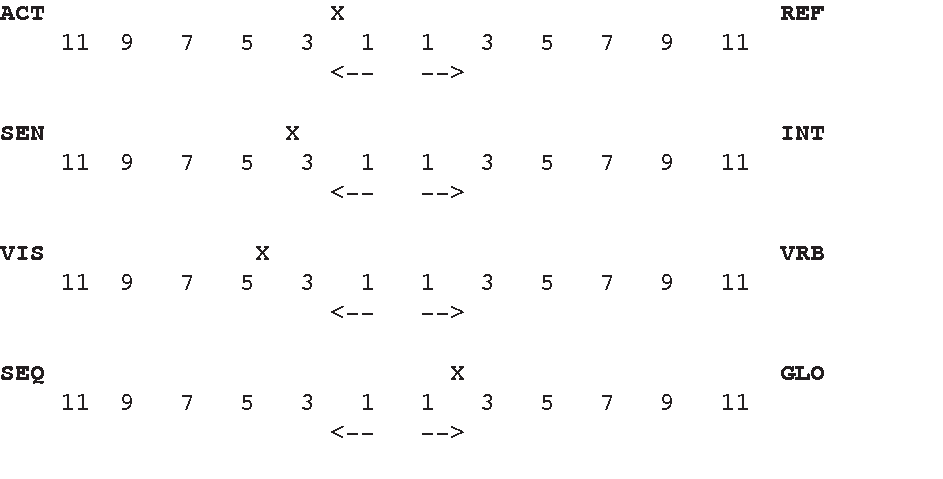
\includegraphics[width=9cm]{figures/overall_learning_style}
\caption{Aggregated Learning Style Preferences of the Class}
\label{fig:learningstyles}
\end{figure}

\subsection*{Discussion of Experiment}
The results show that the students in the class prefer \textbf{active},  \textbf{sensing}, \textbf{visual}, and \textbf{global} learning styles. Three out of four categories match the statements made by Felder and Silverman. The difference is in the last category, where our experiment shows that the students have a small preference for a global learnering style. The visual/verbal preference contains the most dominant preference.


% Weekly evaluation of the learning activities
\section{Weekly Evaluation of the Learning Activities}
\subsection*{Design of Experiment}

After determining the students' learning style preferences, we need to measure the students' progression. An evaluation of the results of the weekly reflection assignments according to SOLO taxonomy is made in the context of the entire course. Part of the course design is the weekly learning goals, and to evaluate the students progression, a weekly reflection assignment is handed in. The goal of this reflection assignment is for the students to reflect upon the weeks' learning activities and, in the first week, determine their initial knowledge of relevant topics. Furthermore, these assignments will provide insight into the students' progression. The assignment contains between three and seven questions. The questions are all asked as open-ended questions, and the students are provided with a text field to input their thoughts. \\

\noindent\textbf{Test Protocol}\\
The questionnaires are released to the students in the last hour of the last lecture of every module. Below is the determined test protocol for each module. The lecture content of Module 6 is prepared by Christoffer Werge, another master's thesis student, and is, therefore, not a part of this master's thesis. \\

\noindent\textit{Reflection before the course}\\
\vspace{-5mm}
\begin{enumerate}
    \setlength\itemsep{0.05em}
  \item What is cloud computing?
  \item What is a distributed system?
  \item What is cluster computing?
  \item What is virtualization?
  \item Describe some benefits and liabilities of sequential vs. parallel execution
  \item Describe your understanding of possible error in communicating over a network
  \item Describe your understanding of resilience in a system
\end{enumerate}

\noindent\textit{Module 1 - Course introduction, Cloud computing, frameworks}\\

\vspace{-5mm}
\begin{enumerate}
\setlength\itemsep{0.05em}
  \item What challenges do you see in cloud computing and microservice architecture?
  \item What would you say a cluster consist of?
  \item What benefits and drawbacks do you see in a microservice architecture compared to a monolithic architecture?
\end{enumerate}

\noindent\textit{Module 2 - Docker lightweight containers}\\

\vspace{-5mm}
\begin{enumerate}
\setlength\itemsep{0.05em}
  \item Describe with your own words the benefits and drawbacks of virtualization in general
  \item Describe with you own words, the difference between Containers and Virtual Machines on Hypervisors
  \item Describe with your own words, benefits and drawbacks of Docker containers
  \item Describe with your own words how Docker fits into a microservice architecture
\end{enumerate}


\noindent\textit{Module 3 - Kubernetes cluster manangement}\\

\vspace{-5mm}
\begin{enumerate}
\setlength\itemsep{0.05em}
    \item Describe the connection between Docker and Kubernetes
    \item Describe with your own words how Kubernetes orchestrates containers
    \item Describe with your own words the benefits and drawbacks of using a cluster management system such as Kubernetes
    \item How did workshop help you understand this week's topic
\end{enumerate}

\noindent\textit{Module 4 - Resilience and load testing}\\

\vspace{-5mm}
\begin{enumerate}
\setlength\itemsep{0.05em}
    \item Describe in your own words what resilience is and provide a couple of examples
    \item How did circuit breakers and replications affect the resilience of the services in the workshop?
    \item How did the workshop help you understand this week's topic?
    \item For what purposes would you use unit testing, load testing, and stress testing respectively?
\end{enumerate}

\noindent\textit{Module 5 - Project work and external presentation}\\

\vspace{-5mm}
\begin{enumerate}
\setlength\itemsep{0.05em}
    \item Describe the process of deploying applications into Kubernetes, and how (if) the ideas of automation pipelines can help?
    \item Describe with your own words the relationship between Microservices, Docker, Kubernetes, and Continuous Delivery
    \item Compare the course content to the real-world perspective described by the external presenter. How does it relate?
\end{enumerate}

\noindent\textit{Module 7 - Service Discovery and project presentations}\\

\vspace{-5mm}
\begin{enumerate}
\setlength\itemsep{0.05em}
    \item Describe the role of service discovery in relation to Docker, Kubernetes, and microservices
    \item Describe the benefits and drawback of having an IP per pod (Kubernetes)
    \item Compare how communication between two pods is performed with or without Kubernetes DNS
\end{enumerate}

\noindent\textbf{Metrics} \\
Since the questions are open-ended, the metrics will be a formative evaluation. The goal is to get an insight in the students' mental models and categorize them using  SOLO taxonomy. The metric is a classification of the answers in relation to the entire course content. \\

\noindent\textbf{Data Basis} \\
The data basis is varying from week to week (Table~\ref{table:weeklyevaluation}).


\subsection*{Results of Experiment}
The overall evaluation of the students' progression in the context of the overall course content is displayed in Table~\ref{table:weeklyevaluation}. As mentioned, Module 6 is out of the scope of this master's thesis. Furthermore, the hand-in process of Module 7 reflections is due on the date of handing in this master's thesis, and is, therefore, not included in this report.

\begin{table}[H]
\centering

\begin{tabular}{|l|l|l|}
\hline
\rowcolor[HTML]{EFEFEF} 
\textbf{Module}                           & \textbf{Responses}          & \textbf{Stage} \\ \hline
0: Before the course                                 & 17   & Prestructural  \\ \hline
1: Course introduction, Cloud computing, frameworks & 13 & Unistructural  \\ \hline
2: Docker lightweight containers                   & 11 & Unistructural  \\ \hline
3: Kubernetes cluster manangement                 & 10  & Multistructural\\ \hline
4: Resilience and load testing                    & 9  & Multistructural            \\ \hline
5: Project work and external presentation        & 10   & Relational            \\ \hline
\end{tabular}
\caption{Weekly Evaluation of Questionnaires (SOLO)}
\label{table:weeklyevaluation}
\end{table}

\noindent\textbf{Evaluation of Module 0: Before the course} \\
As seen from Table~\ref{table:weeklyevaluation} we evaluate the students' stage before the course to be in the \textit{prestructural stage}. The basis for this result stems from examining and evaluating the answers of 17 students to a total of seven asked questions. A common theme, when asked about what cloud computing is, was to some degree wrong answers and misconceptions of what cloud computing is, e.g. \textit{"As far as i know, cloud computing is a system (and/or) application hosted in the cloud"}. The prestructural stage is the stage of ignorance, and this was also clearly stated by some of the students, e.g. \textit{"I don't know"}. The overall evaluation of the questionnaire and the students' stage before the course is, therefore, \textit{prestructural}. \\

\noindent\textbf{Evaluation of Module 1: Course introduction, Cloud computing, frameworks}\\ 
The questionnaire of Module 1 contained three questions with a total of 13 students completing the assignment. The questions asked focused on the main topics of the week, namely cloud computing and specifically microservices architecture. The evaluation of the answers supplied by the students show a transition from the \textit{prestructural} stage to the \textit{unistructural} stage. A common theme is small simple observations like \textit{"Connections between devices. Being consistent with interfaces"} when asked about the challenges in cloud computing and microservice architecture. However, two answers show a higher degree of understanding and use of vocabulary to describe the challenges, and are closer to the \textit{multistructural stage}. The unified evaluation shows a transition from the \textit{prestructural} stage to the \textit{unistructural} stage.  \\ 

\noindent\textbf{Evaluation of Module 2: Docker lightweight containers}\\ 
In Module 2, the students have not progressed in terms of the SOLO taxonomy stages. The students show an individual understanding of the topic of the week, however, the bigger picture is still missing. The students demonstrate their understanding of Docker containers in conjunction with microservices. In the context of the entire course, the relations are not demonstrated. It is a natural stage to be in at this point in the course. One student actually demonstrate the ability to look forward, and makes the connection to the following week, \textit{"Docker helps us deploy the microservices in an easy manner, especially when Kubernetes starts getting involved, which will hopefully grant a better overview of running services etc."}. Despite this observation the majority of the answers still shows small misconceptions and \textit{unistructural} responses such as \textit{"Its smart because its not hardware dependent"}. The overall evaluation of Module 2 results in the \textit{unistructural} stage. \\

\noindent\textbf{Evaluation of Module 3: Kubernetes cluster manangement}\\ 
The evaluation of Module 3 results in a transition from the \textit{unistructural} stage to the \textit{multistructural} stage. This transition is demonstrated with responses such as \textit{"Docker is used to pack software into containers which afterwards can be pushed to the docker hub. Kubernetes responsibility is to run the containers and distribute them among one or multiple machines in a cluster."} The students in general demonstrate the ability to understand the topics in isolation. Simple connections are made between different introduced topics of the course. However, some are still providing \textit{unistructural} answers such as \textit{"Kubernetes manages the docker containers"}. The overall evaluation results in a transition from the \textit{unistructural} stage to the \textit{multistructural stage}. \\

\noindent\textbf{Evaluation of Module 4: Resilience and load testing}\\ 
No progression is made from Module 3 to Module 4 in terms of SOLO. The number of students handing in this assignment were only a total of 9. The answers are fairly short, but a few students demonstrate the \textit{multistructural} understanding with answers such as \textit{"You would unit test single services to check if the service is working as intended. Load testing to see if the system works as indended under normal or slightly above normal load. Stress testing to see how the system reacts under massive load and how it recovers from the problems that arise."}  The overall evaluation of Module 2 results in the \textit{multistructural} stage. \\

\noindent\textbf{Evaluation of Module 5: Project work and external presentation}\\ 
The evaluation of Module 5 results in a transition from the \textit{multistructural} stage to the \textit{relational} stage. This transition is demonstrated by multiple answers describing the relationship between many of the topics in the course, e.g. \textit{"Microservices is the idea of having Small independant applications instead of Big monoliths. They are usually used together with docker. Docker containerize your app making them self contained in the Sense that they have their own enviroment Inside the containers. Kubernetes is a container management system that helps with stuff like resilience by replicating and restoring downed applications. Continous delivery in this context is about being able to upgrade these small containers individually instead of a monolith where you have to do the big bang deployment"}. In general, the students have submitted longer and more detailed descriptions and the overall evaluation of the week is a transition from the \textit{multistructural} stage to the \textit{relational} stage.


\subsection*{Discussion of Experiment}
As seen from the results in Table~\ref{table:weeklyevaluation} the students' progression is increasing in terms of the stages in SOLO taxonomy. The students started out before the course, as expected, knowing little about the concepts, and in Module 5 demonstrates the ability to analyze and compare different topics. \\

\noindent
The number of students submitting answers has led to a smaller respondet pool than expected. For the majority of the assignments slightly over half of the 18 students are handing in the reflection assignments. The validity of the experiment can be questioned, because of the small number of respondents. However, the assignments have been an important tool in getting insights into the students' progression and knowledge from module to module. If it is clear from the assignments that a topic has been misunderstood, we have the possibility of correcting the mistake in the following module. \\

\noindent
Another topic of discussion is the evaluation of answers provided by the students. Many answers are fairly short, and can be categorized as prestructural, or at best unistructural. A reason for these types of answers is properly related to the nature of the assignment. Even though the students are told the assignments are mandatory, they consider them optional. This may be because of the formative and qualitative nature of the assignments, and that it is purely based on their thoughts and not actual theory. The students are asked not to use any tools, and only answer to the best of their knowledge. Furthermore, they are told that they are not judged by their answers.

% Weekly evaluation of KubeCloud
\section{Weekly Evaluation of KubeCloud}
\subsection*{Design of Experiment}
To determine KubeCloud's usefulness as a learning object, an experiment covering the students' experience with it and perception of it is designed. \\

\noindent
The questionnaires from the previous and this experiment are combined in the weekly reflection exercises. Questions about KubeCloud's role are asked to disclose the students' mental models during the course. The answers will be used to clarify and classify KubeCloud's role as a learning object according to existing theories for learning objects.

\subsubsection*{Test Protocol}
The questions for the questionnaires are presented below. The questionnaires are sent out in the last hour of Module 2, Module 3, and Module 4. In Module 1 a question is asked immediately after a demonstration of parallel workloads distributed on a Raspberry Pi cluster. The Raspberry Pi cluster in Module 1 is not KubeCloud, and the other cluster only appears to visualize the benefit and drawbacks of distributing workloads across multiple Raspberry Pis. The answers are categorized and compared to the theories presented in Chapter~\ref{chap_fundamentals_learning}. \\

\noindent
\textit{Module 1}
\begin{enumerate}
\setlength\itemsep{0.05em}
	\item Did the cluster give you a better understanding of cluster computing?
\end{enumerate}

\noindent
\textit{Module 2 reflection}
\begin{enumerate}
\setlength\itemsep{0.05em}
	\item Describe how (if) the Raspberry Pi Cluster helped your learning
\end{enumerate}

\noindent
\textit{Module 3 reflection}
\begin{enumerate}
\setlength\itemsep{0.05em}
	\item Describe how (if) the Raspberry Pi Cluster helped your learning
	\item Describe how the Kubernetes visualization tool helped your learning
	\item How did the cluster help you understand the scheduling done by Kubernetes?
	\item How did the workshop help you understand this week's topic? 
\end{enumerate}

\noindent
\textit{Module 4 reflection}
\begin{enumerate}
\setlength\itemsep{0.05em}
	\item Describe how (if) the Raspberry Pi Cluster helped your learning
	\item Did the cluster support your understanding of what resilience is? If yes, how?
\end{enumerate}


\subsubsection*{Metrics}
Since the questions are open-ended questions, the metrics will cover a qualitative, formative evaluation.
\\
Statements from the students are expected to confirm the value of the cluster as a learning object and help classify the type of learning object according to Churchill's classifications. The cluster's role as a mediating tool as described in activity theory is also expected to be seen from the answers. Lastly, the importance of an object to explore and experiment with, as described in constructivist learning theory, is expected to be observed in the students' answers.

\subsubsection*{Data Basis}
The data basis is varying from week to week (Table~\ref{table:weeklyevaluation}).


\subsection*{Results of Experiment}
The responses from each module show that the students' responses contain different characteristics of learning objects. The usefulness of the cluster in regards to learning is indicated in the responses, but generalized conclusions cannot be drawn from the answers. This section will present the main points from the questions. The raw data responses and an analysis can be found in Attachment 7. \\

\noindent
\textbf{Evaluation of Module 1: Course introduction, Cloud computing, frameworks} \\
After demonstrating distributed workloads on a cluster (not KubeCloud), 15 of 17 students stated that it provided them with a better understanding of cluster computing. \\

\noindent
\textbf{Evaluation of Module 2: Docker lightweight containers} \\
% Question 5: Describe how (if) the Raspberry Pi Cluster helped your learning
The students were asked whether KubeCloud helped their learning. Six of eight students expressed, either directly or indirectly, that the cluster was a help e.g. because it visualized or illustrated something for them. Two students expressed that it did not help them. They point out that the workshop could have been done without the cluster, and that the cluster will be more useful when Kubernetes is introduced. The largest other category found in the answers was a description of the cluster as a 'scale model' or similar description. The cluster is e.g. referred to as a "remote host" and "a small-scale model". Furthermore, enthusiasm was present in two of the responses since running containers on the cluster is called 'cool' and because 'motivation' is mentioned. \\

\noindent
\textbf{Evaluation of Module 3: Kubernetes cluster manangement}\\
%Question 3: Describe how (if) the Raspberry Pi Cluster helped your learning
\noindent
All seven students reported that KubeCloud helped their learning in this module. The help from the visualization was mentioned in all the responses. How it helped to understand the location of the pods was described in different ways. A student sums up: \textit{"The cluster illustrates the purpose and setup visually in a nice way. It is very hands on to work with these compared to some cloud setup where the actual servers in the cluster are hidden away"}.
%Question 4: Describe how the Kubernetes visualization tool helped your learning
% Ikke rigtigt noget ekstra end det tidligere.
% Question 5: How did the cluster help you understand the scheduling done by Kubernetes?
\noindent
The students did, however, not agree on whether the cluster helped them understand the scheduling done in Kubernetes. Four students either did not see it as a help or did not understand the scheduling happening in the cluster. Three students described how it helped them know which Raspberry Pi, pods were being scheduled on. \\
%Question 7: How did the workshop help you understand this weeks’ topic?
\noindent
When asked about the workshop, three of the students mentioned that they liked the \textit{"hands on"} or practical application of the theory. Statements such as \textit{"hands on is the best learning tool"} and \textit{"Hands on is all ways good."} supports this. The workshop format was both complimented and criticized. Sharing a cluster was pointed out as a drawback by a student. A student pointed out that the one at the pc \textit{"got most out of the workshop"}. \\

\noindent
\textbf{Evaluation of Module 4: Resilience and load testing} \\
\noindent
%Question 4: Describe how (if) the Raspberry Pi Cluster helped your learning
Seven of eight students stated that KubeCloud helped their learning in this module. The last student referred to another question.
Six of the students mentioned that they liked the physical aspect of the exercise or the possibility of pulling the network cable. A student describes: \textit{"[...] This helped understading how a part of a system could be down, and other parts can take over the service"}.
%Question 5: Did the cluster support your understanding of what resilience is? If yes, how?
\noindent
When asked if KubeCloud supported their understanding of resilience, seven of nine students said it did. Six students mentioned that their understanding of the mechanisms and concepts of Kubernetes were supported by the cluster. Lastly, four students used the word recover and two more described the concept. \\

\subsection*{Discussion of Experiment}
\noindent
In Module 2, similarities are seen between KubeCloud and Churchill's \textit{practice object} which is a \textit{"representation that allows practice and learning of certain procedures"}. The criticism of the exercises being possible without the cluster is fair. The inconvenience of Docker on ARM is unfortunate. However, Docker is necessary to use Kubernetes in Module 3. Motivation is seen from the results which is in agreement with Hein's emphasis on motivation and Piaget's emphasis on play. \\

\noindent In Module 3, the importance of the visualization is seen. This is in agreement with Felder and Silverman's research on engineering students being visual learners. The sensory preference is also seen in some of the students, who like the hands-on aspect. Furthermore, that the cluster is shared in groups during workshops is criticized. This is an interesting point of view compared to mediating tools from activity theory. The students are, according to one student, not able to attain the same knowledge during the workshops since the cluster (mediating tool) is not equally available to all members of the group. We agree that the workshop format leads to one person typing in the commands, however, this limitation is only due to the format of the workshop. KubeCloud allows students to connect and deploy services independently.  \\

\noindent
In Module 4, many of the students had positive feedback and highlighted the physical aspect and the ability to pull the network cable and see the reaction. Again, the sensory and visual preference is reflected.

% Overall evaluation of the learning activities
\section{Overall Evaluation of the Learning Activities}
\subsection*{Design of Experiment}
To combine the previous two experiments and to evaluate the students' overall outcome of the designed learning activity, a last experiment is conducted. The goal of this experiment is to quantify the students' overall thoughts and view on the learning experience they have been exposed to. \\

\noindent\textbf{Test Protocol} \\
The questions for the overall evaluation of the tangible cloud computing cluster and the course in general are joined. The questionnaire is sent out in the beginning of the last module of the course and the students are given 20 minutes to complete the questionnaire. The questionnaire is divided into two parts; one focusing on the effect of using a cluster, and one focusing on the course.

\noindent\textit{Statements relating to the course design:}
%\vspace{-3mm}
\noindent\begin{enumerate}
	\item\textbf{Course structure}
	\vspace{-4mm}
	\begin{enumerate}
	    \setlength\itemsep{0.05em}
		\item The distribution of theory and practical work was suitable
		\item The order of the topics was well-planned
		\item The problem based project allowed me to apply the concepts and theories
		\item The workshops provided me with the necessary skills for the project work
	\end{enumerate}
	
	\item\textbf{Materials}
	\vspace{-4mm}
	\begin{enumerate}
	    \setlength\itemsep{0.05em}
		\item The reading and video materials provided me with the essentials for each module
		\item The slides covered the necessary theory
		\item The blog (rpi-cloud.com) helped me getting started with Spring Boot and Spring Cloud
	\end{enumerate}
	
	\item\textbf{Comparision}
	\vspace{-4mm}
	\begin{enumerate}
	    \setlength\itemsep{0.05em}
		\item In comparison with other courses my overall rating of the course is
	\end{enumerate}
\end{enumerate}


\noindent\textbf{Metrics} \\
All questions are asked as statements that the student can rate their compliance in terms of a five-level Likert scale. (1: Strongly disagree; 2: Disagree; 3: Neutral; 4: Agree; 5: Strongly Agree). All questions are related to a top-level classification in order to provide a summarized result. The categories of interest are a rating of the \textit{Course structure}, a rating of the supplied \textit{Materials}, and a rating of the designed learning activity in \textit{Comparison} with other courses. \\
\noindent 

\noindent\textbf{Data Basis}\\
The data basis consists of 16 students as described in the introduction of this chapter.

\subsection*{Results of Experiment}
The overall evaluation of the designed learning activity is displayed in the tables below. The results of each of the three metrics is presented below. Further details can be found in Appendix~\ref{appendix_overall_evaluation}. Note: Statement (Comparison) is asked as a rating from very bad to very good.

\renewcommand*{\arraystretch}{1.7}
\begin{table}[H]
\centering
\begin{tabular}{|p{9cm}|p{0.8cm}|p{0.8cm}|p{0.8cm}|p{0.8cm}|p{0.8cm}|}
\hline
\rowcolor[HTML]{EFEFEF} 
\textbf{Statements (Course structure)}             & \textbf{1} [\%] & \textbf{2} [\%] & \textbf{3} [\%] & \textbf{4} [\%] & \textbf{5} [\%]   \\ \hline
The distribution of theory and practical work was suitable		& 0 & 6.3 & 12.5 & 43.8 & 37.5    	 	\\ \hline
The order of the topics was well-planned		& 0 & 12.5 & 12.5 & 50 & 25    	 	\\ \hline
The problem based project allowed me to apply the concepts and theories		& 0 & 0 & 18.8 & 43.8 & 37.5    	 	\\ \hline
The workshops provided me with the necessary skills for the project work		& 0 & 18.8 & 25 & 31.3 & 25    	 	\\ \hline
\rowcolor[HTML]{EFEFEF} 
\textbf{Total}             	& \textbf{0}	& \textbf{9.4}	& \textbf{17.2}	 & \textbf{42.2} & \textbf{31.3}   \\ \hline
\end{tabular}
\caption{Overall Evaluation of the Designed Learning Activity: Course Structure}
\label{table:overallevaluationlearningactivitycoursestructure}
\end{table}



\begin{table}[H]
\centering
\begin{tabular}{|p{9cm}|p{0.8cm}|p{0.8cm}|p{0.8cm}|p{0.8cm}|p{0.8cm}|}
\hline
\rowcolor[HTML]{EFEFEF} 
\textbf{Statements (Materials)}             & \textbf{1} [\%] & \textbf{2} [\%] & \textbf{3} [\%] & \textbf{4} [\%] & \textbf{5} [\%]   \\ \hline
The reading and video materials provided me with the essentials for each module		& 0 & 6.3 & 25 & 31.3 & 37.5    	 	\\ \hline
The slides covered the necessary theory		& 0 & 0 & 18.8 & 50 & 31.3    	 	\\ \hline
The blog (rpi-cloud.com) helped me getting started with Spring Boot and Spring Cloud		& 0 & 12.5 & 18.8 & 37.5 & 31.3    	 	\\ \hline
\rowcolor[HTML]{EFEFEF} 
\textbf{Total}             	& \textbf{0} & \textbf{6.3}  & \textbf{20.9}  & \textbf{39.6}  & \textbf{33.4}   \\ \hline
\end{tabular}
\caption{Overall Evaluation of the Designed Learning Activity: Materials}
\label{table:overallevaluationlearningactivitymaterials}
\end{table}



\begin{table}[H]
\centering
\begin{tabular}{|p{9cm}|p{0.8cm}|p{0.8cm}|p{0.8cm}|p{0.8cm}|p{0.8cm}|}
\hline
\rowcolor[HTML]{EFEFEF} 
\textbf{Statement (Comparison)}             & \textbf{1} [\%] & \textbf{2} [\%] & \textbf{3} [\%] & \textbf{4} [\%] & \textbf{5} [\%]   \\ \hline
In comparison with other courses my overall rating of the course is		  &  0 & 6.3 & 0 & 50 & 43.8    	 	\\ \hline
\rowcolor[HTML]{EFEFEF} 
\textbf{Total}             	& \textbf{0} & \textbf{6.3} & \textbf{0} & \textbf{50} & \textbf{43.8}   \\ \hline
\end{tabular}
\caption{Overall Evaluation of the Designed Learning Activity: Comparison}
\label{table:overallevaluationlearningactivitycomparison}
\end{table}

\subsection*{Discussion of Experiment}
The overall rating of the designed learning activity is that 75.8\% of the students either agree or strongly agree with the statements. The workshops scored lowest within the category \textit{Course structure} with 56.3\% agreeing or strongly agreeing. Nearly one out of five disagreed with \textit{The workshops provided me with the necessary skills for the project work}. A student expressed that the workshops were too simple or linear and further adds: \textit{"I think the workshops could be a little more free to experiments to increase the understanding of the concepts."}. These results indicate that the workshops should have allowed for more experimentation as described in constructivist learning theory. However, the overall choice of PBL seems suitable in relation to the project work. A student points out one of the core theories in constructivist learning theory: \textit{"The real understanding of the concepts arrived when we worked on the project."}. Another key finding  pointed out by a student is the order of the last two subjects DNS and service discovery. A better structure would have been placing the external presentation in one of the last modules. The initial point behind this was to make room for group work and give the students the ability to leverage some of the concepts presented, such as automation with Jenkins.\\

\noindent
Lastly, in comparison with other courses 93.8\% of the students rate the designed course as either good or very good. This result suggests that there is an interest for these topics among the students. The students point out the relevance of the topics: \textit{"Much of this could very well be mandatory on the IKT engineering studies as the distributed systems are growing and the standardized monolithic architectures are disappearing from the more modern and scalable applications."}. One student mentions that the course introduced many new concepts which resulted in a "huge" workload for some of the students.

% Overall evaluation of KubeCloud
\section{Overall Evaluation of KubeCloud}

\subsection*{Design of Experiment}
The design of the experiment of the overall evaluation of KubeCloud is as mentioned evaluated in conjunction with the overall evaluation of the learning activities.\\

\noindent\textbf{Test Protocol} \\
The test protocol is the same as described in the \textit{Overall evaluation of the learning activities}.

\noindent\textit{Statements relating to the tangible cluster}
%\vspace{-3mm}
\begin{enumerate}
	\item\textbf{Physical appearance of the cluster:}
	\vspace{-4mm}
	\begin{enumerate}
	    \setlength\itemsep{0.05em}
		\item The cluster provided me a better understanding of what a cloud consists of
		\item The physicality of the cluster provided a better understanding of errors in distributed systems (e.g. pulling the network cable)
		\item The physical design of the cluster gave me associations to a real server rack
	\end{enumerate}
	
	\item\textbf{Group activity}
	\vspace{-4mm}
	\begin{enumerate}
	    \setlength\itemsep{0.05em}
		\item The cluster allowed me to experiment
		\item The cluster initiated group discussions
	\end{enumerate}
	
	\item\textbf{Visualization}
	\vspace{-4mm}
	\begin{enumerate}
	    \setlength\itemsep{0.05em}
		\item The cluster combined with the visualizer helped me understand the concepts of the cluster
		\item The cluster combined with the visualizer helped me understand the how errors are handled
	\end{enumerate}
	
	\item\textbf{Movitation}
	\vspace{-4mm}
	\begin{enumerate}
	    \setlength\itemsep{0.05em}
		\item The use of a cluster increased my motivation
		\item The cluster motivated me to do out of curriculum experimentation
		\item The cluster was a fun and playful way of learning the concepts
	\end{enumerate}
	
	\item\textbf{Relation to the real world}
	\vspace{-4mm}
	\begin{enumerate}
	    \setlength\itemsep{0.05em}
		\item Using a cloud provider (e.g. Google Container Engine) instead of a hands-on tool would have improved my learning
		\item The cluster represents a small-scale datacenter
		\item The cluster improved my skills in relevant technologies
	\end{enumerate}
	 
\end{enumerate}

\noindent\textbf{Metrics} \\
All questions are asked as statements that the student can rate their compliance in terms of a five-level Likert scale. (1: Strongly disagree; 2: Disagree; 3: Neutral; 4: Agree; 5: Strongly Agree). All questions are related to a top-level classification in order to provide a summarized result. The categories of interest are a rating of the \textit{Physical appearance of the cluster}, a rating of KubeCloud's role during \textit{Group Activity}, a rating of the \textit{Visualization} aspects provided by KubeCloud, a rating of KubeCloud's ability to \textit{Motivate}, and a rating of KubeCloud's \textit{Relation to the real world}. \\
\noindent 


\noindent\textbf{Data Basis}\\
The data basis consists of 16 students as described in the introduction of this chapter.


\subsection*{Results of Experiment}
The overall evaluation of KubeCloud is displayed in the tables below. The results of each of the three metrics is presented below. Further details can be found in Appendix~\ref{appendix_overall_evaluation}.




\begin{table}[H]
\centering
\begin{tabular}{|p{9cm}|p{0.8cm}|p{0.8cm}|p{0.8cm}|p{0.8cm}|p{0.8cm}|}
\hline
\rowcolor[HTML]{EFEFEF} 
\textbf{Statements (Physical appearance)}             & \textbf{1} [\%] & \textbf{2} [\%] & \textbf{3} [\%] & \textbf{4} [\%] & \textbf{5} [\%]   \\ \hline
The cluster provided me a better understanding of what a cloud consists of		 &     0 & 0 & 0 & 56.3 & 43.8 	 	\\ \hline
The physicality of the cluster provided a better understanding of errors in distributed systems (e.g. pulling the network cable)		&    6.3 & 0 & 6.3 & 56.3 & 31.3 	 	\\ \hline
The physical design of the cluster gave me associations to a real server rack		&  0 & 6.3 & 12.5 & 37.5 & 43.8   	 	\\ \hline
\rowcolor[HTML]{EFEFEF} 
\textbf{Total}             	& \textbf{2.1} & \textbf{2.1} & \textbf{6.3} & \textbf{50} & \textbf{39.6}   \\ \hline
\end{tabular}
\caption{Overall Evaluation of KubeCloud's Physical Appearance}
\label{table:overallevaluationclusterphysical}
\end{table}

\vspace{-1mm}

\begin{table}[H]
\centering
\begin{tabular}{|p{9cm}|p{0.8cm}|p{0.8cm}|p{0.8cm}|p{0.8cm}|p{0.8cm}|}
\hline
\rowcolor[HTML]{EFEFEF} 
\textbf{Statements (Group activity)}             & \textbf{1} [\%] & \textbf{2} [\%] & \textbf{3} [\%] & \textbf{4} [\%] & \textbf{5} [\%]   \\ \hline
The cluster allowed me to experiment		 & 0 & 6.3 & 18.8 & 37.5 & 37.5    	 	\\ \hline
The cluster initiated group discussions		&   12.5 & 25 & 18.8 & 12.5 & 31.3  	 	\\ \hline
\rowcolor[HTML]{EFEFEF} 
\textbf{Total}             	 & \textbf{6.3} & \textbf{15.7} & \textbf{18.8} & \textbf{25} & \textbf{34.4}   \\ \hline
\end{tabular}
\caption{Overall Evaluation of KubeCloud in Relation to Group Activity}
\label{table:overallevaluationclustergroup}
\end{table}

\vspace{-5mm}

\begin{table}[H]
\centering
\begin{tabular}{|p{9cm}|p{0.8cm}|p{0.8cm}|p{0.8cm}|p{0.8cm}|p{0.8cm}|}
\hline
\rowcolor[HTML]{EFEFEF} 
\textbf{Statements (Visualization)}             & \textbf{1} [\%] & \textbf{2} [\%] & \textbf{3} [\%] & \textbf{4} [\%] & \textbf{5} [\%]   \\ \hline
The cluster combined with the visualizer helped me understand the concepts of the cluster		 &  0 & 0 & 6.3 & 43.8 & 50     	 	\\ \hline
The cluster combined with the visualizer helped me understand the how errors are handled		&     0 & 6.3 & 31.3 & 12.5 & 50	 	\\ \hline
\rowcolor[HTML]{EFEFEF} 
\textbf{Average}             	 & \textbf{0} & \textbf{3.2} & \textbf{18.8} & \textbf{28.2} & \textbf{50}   \\ \hline
\end{tabular}
\caption{Overall Evaluation of KubeCloud in Relation to Visualization}
\label{table:overallevaluationclustervisualization}
\end{table}

\vspace{-5mm}

\begin{table}[H]
\centering
\begin{tabular}{|p{9cm}|p{0.8cm}|p{0.8cm}|p{0.8cm}|p{0.8cm}|p{0.8cm}|}
\hline
\rowcolor[HTML]{EFEFEF} 
\textbf{Statements (Motivation)}             & \textbf{1} [\%] & \textbf{2} [\%] & \textbf{3} [\%] & \textbf{4} [\%] & \textbf{5} [\%]   \\ \hline
The use of a cluster increased my motivation		 & 0 & 0 & 43.8 & 43.8 & 12.5	 	\\ \hline
The cluster motivated me to do out of curriculum experimentation	& 6.3 & 31.3 & 37.5 & 25 & 0 	 	\\ \hline
The cluster was a fun and playful way of learning the concepts	& 0 & 6.3 & 18.8 & 56.3 & 18.8   	 	\\ \hline
\rowcolor[HTML]{EFEFEF} 
\textbf{Total}             	 & \textbf{2.1} & \textbf{12.5} & \textbf{33.4} & \textbf{41.7} & \textbf{10.4}   \\ \hline
\end{tabular}
\caption{Overall Evaluation of KubeCloud in Relation to Motivation}
\label{table:overallevaluationclustermotivation}
\end{table}

\vspace{-5mm}

\begin{table}[H]
\centering
\begin{tabular}{|p{9cm}|p{0.8cm}|p{0.8cm}|p{0.8cm}|p{0.8cm}|p{0.8cm}|}
\hline
\rowcolor[HTML]{EFEFEF} 
\textbf{Statements (Relation to real world)}             & \textbf{1} [\%] & \textbf{2} [\%] & \textbf{3} [\%] & \textbf{4} [\%] & \textbf{5} [\%]   \\ \hline
Using a cloud provider (e.g. Google Container Engine) instead of a hands-on tool would have improved my learning		 & 0 & 25 & 31.3 & 43.8  & 0	 	\\ \hline
The cluster represents a small-scale datacenter		& 0 & 0 & 37.5 & 50 & 12.5 	\\ \hline
The cluster improved my skills in relevant technologies		& 0 & 0 & 25 & 62.5 & 12.5 	 	\\ \hline
\rowcolor[HTML]{EFEFEF} 
\textbf{Total}             	& \textbf{0} & \textbf{8.3} & \textbf{31.3} & \textbf{52.1} & \textbf{8.3}   \\ \hline
\end{tabular}
\caption{Overall Evaluation of KubeCloud in Relation to the Real World}
\label{table:overallevaluationclusterrealworld}
\end{table}

\noindent
Note: The result of the first question (Table~\ref{table:overallevaluationclusterrealworld}) has been reversed due to the negated form of the statement.
\renewcommand*{\arraystretch}{1.8}

\subsection*{Discussion of Experiment}
The overall rating of KubeCloud is that 67.8\% of the students agree or strongly agree with the statements. A key finding, within the physical appearance category of questions asked, is that the cluster supports the students' understanding of what cloud computing consists of. Furthermore, a surprising finding is that one student rates KubeCloud's ability to provide an understanding of errors in distributed systems to strongly disagree. However, 87.6\% of the students either agree or strongly agree with the statement that KubeCloud provides a better understanding of errors in distributed systems. \\

\noindent
KubeCloud was placed at a table in the front row of the classroom, and a physical distance between the groups and the clusters was present. One student points out: \textit{"The cluster was for a long time this "wierd thing" which we were mostly scared of breaking - which led to only doing things to it described in workshops."}. The length of the network cables for each cluster introduced this limitation. Optimally, each group should have their cluster right in front of them instead of this physical distance. The benefit of having the physically located on the table in front of them would have minimized the mental gap. The students did not agree on KubeCloud's ability to initiate group discussions. 37.5\% disagreed or strongly disagreed whereas 43.8\% agreed or strongly agreed. A reason for this disagreement could be the students' delegation of tasks internally in the groups, which led to a parallel development of the project work. This way of decomposing the project was also observed from our facilitating role. \\

\noindent
The visualization category is among the highest rated in the evaluation of KubeCloud with 78.2\% of the students either agreeing or strongly agreeing with the statements. The visualizer provided the students with a better understanding of the concepts of the KubeCloud and how errors are handled in Kubernetes. However, as one student points out: \textit{"It's unfortunate that the visualizer was so bugged."}. The visualization tool, even with our improvements, is still not performant enough. \\

\noindent
The motivation category received the lowest agreement with the statements. A reason for this relatively low score is that 37.6\% students disagreed or strongly disagreed with the statement: \textit{The cluster motivated me to do out of curriculum experimentation}. This is a bold question since the students are asked whether or not they are motivated to do out of curriculum experimentation. 25\% of the students answer that they agree with the statement, and have been doing extra activities. A key finding in the motivational category confirms our previously described limitation of Docker and ARM architectures: \textit{"The cluster made the workshops and project more real compared to using a cloud cluster. Too bad the ARM architecture broke the seamless experience of using docker."}. This is unfortunate but to illustrate and improve the students' skills Docker on ARM is still a valid solution since the API is the same. \\

\noindent
The most significant finding in the relation to the real world category is the trade-off between using the cluster opposite a cloud provider in relation to Docker. The limitation of Docker on ARM does not exist at the cloud provider, but the abstractions and understanding of the cluster are harder to grasp. A student points out: \textit{"Cloud providers would have made the user of Docker more meaningful, but not the cluster understanding."}. Furthermore, according to the students, KubeCloud provided them with the ability to improve their skills with relevant real-world technologies.



%%%%%%%%%%%%%%%%%%%%%%%%%%%% FOER %%%%%%%%%%%%%%%%%%%%%%%%%%
%\section{Design of experiments}
%%!TEX root = ../../master.tex
\noindent\textbf{Test protocol}\\
TBD \\ 
 
\noindent\textbf{Metrics} \\
TBD \\

\noindent\textbf{Data basis} \\

%
%\section{Results}
%%!TEX root = ../../master.tex

\subsection*{Experiment 2.1 - Course}
This section will present the results of the performed experiments done with regards to the teaching and the course.






 


\subsection*{Experiment 2.2 - Tangible cloud cluster}



\subsection*{Experiment 2.3 - Overall evaluation of the learning experience}

%
%
%\section{Discussion}
%\subsection*{Experiment 2.1 - Course}
%\subsection*{Experiment 2.2 - Tangible cloud cluster}
%\subsection*{Experiment 2.3 - Overall evaluation of the learning experience}
%\subsection*{Overall discussion}

